\documentclass[11pt,a4paper]{article}
\usepackage{amsmath,amssymb}
\usepackage{booktabs}
\usepackage{microtype}
\usepackage{parskip}
\usepackage{tikz}
\usetikzlibrary{arrows.meta,positioning}

\title{Cadmium Experiments\\
  \large Tick-Counter Reordering Study}
\author{Damián Vicino}
\date{2026}

\setlength{\emergencystretch}{3em}

\begin{document}
\maketitle
\tableofcontents
\clearpage

\section{Implementation Notes}
\documentclass[11pt,a4paper]{article}
\usepackage{amsmath,amssymb}
\usepackage{booktabs}
\usepackage{microtype}
\usepackage{parskip}

\title{Cadmium --- Implementation Notes\\
  \large Assumptions and Context Common to All Experiments}
\author{Damián Vicino}
\date{2026}

\begin{document}
\maketitle

This document records the formalism choices, simulator capabilities, and
conventions that apply to every experiment in this repository.
Experiment-specific specs should reference these notes rather than repeat them.

% ─────────────────────────────────────────────────────────────────────────────
\section*{Foundational Reference}

The tick-counter experiment reproduced in this repository originates from:

\begin{quote}
  Damian Vicino, Olivier Dalle, Gabriel A.\ Wainer.
  \textit{A Data Type for Discretized Time Representation in DEVS.}
  SIMUTOOLS 2014. \texttt{hal-01055555}.
\end{quote}

% ─────────────────────────────────────────────────────────────────────────────
\section*{Formalisms Available in Cadmium}

Cadmium implements two related but distinct DEVS-family formalisms.
Each experiment directory states which formalism it targets.

\subsection*{PDEVS — Parallel DEVS}

PDEVS transitions \emph{all} imminent models simultaneously.  At each time
step the set of imminent models $I \subseteq D$ is computed; every model in
$I$ fires its output function $\lambda$ and then its internal transition
$\delta_{\text{int}}$; models not in $I$ that receive routed output undergo
their external transition $\delta_{\text{ext}}$.  When a model is both
imminent and receives external input, the \textbf{confluence function}
$\delta_{\text{con}}$ resolves the two transitions:
\[
  \delta_{\text{con}}(s, e, x) =
    \delta_{\text{ext}}\!\left(\delta_{\text{int}}(s),\; 0,\; x\right)
  \quad \text{(internal-first, the Cadmium default)}
\]

Multiple simultaneous messages are delivered as a \textbf{message bag}
(\texttt{std::vector<T>} per port), allowing many values per port per step.

\subsection*{Classic DEVS — Sequential DEVS}

Classic (sequential) DEVS serialises event processing: at each time step
\emph{exactly one} imminent model transitions.  When more than one model is
scheduled at the same time, the \textbf{SELECT} function breaks the tie:
\[
  \text{SELECT} : 2^D \setminus \{\emptyset\} \to D,\quad
  \text{SELECT}(I) \in I
\]
The chosen model fires; outputs are delivered to influenced models as
\textbf{message boxes} (at most one value per port per step); then time
advances and the next step begins.

\subsection*{Key Differences}

\begin{center}
\begin{tabular}{@{}lll@{}}
  \toprule
  & PDEVS & Classic DEVS \\
  \midrule
  Imminent set   & all simultaneous models & one model (SELECT) \\
  Tie-breaking   & confluence function      & SELECT function \\
  Message carrier & bag (\texttt{vector})  & box (at most one) \\
  Coordinator    & \texttt{pdevs::coordinator} & bespoke per experiment \\
  \bottomrule
\end{tabular}
\end{center}

% ─────────────────────────────────────────────────────────────────────────────
\section*{Typed Port System}

Both formalisms in Cadmium use a \textbf{typed port system}.  Each port is a
distinct C++ type carrying a specific message type; couplings are expressed as
typed \texttt{(sender-port, receiver-port)} pairs verified at compile time.
Port types are declared as:

\begin{itemize}
  \item \texttt{cadmium::out\_port<T>} — output port carrying values of type \texttt{T}
  \item \texttt{cadmium::in\_port<T>}  — input port carrying values of type \texttt{T}
\end{itemize}

Each model declares its ports via \texttt{using input\_ports} and
\texttt{using output\_ports} type aliases.  The compiler rejects any coupling
where the message types do not match.

% ─────────────────────────────────────────────────────────────────────────────
\section*{TIME Type}

Cadmium is parameterised over a \texttt{TIME} template argument that must
satisfy \texttt{cadmium::concepts::Time}: totally ordered, supporting
arithmetic operations, and providing
\texttt{std::numeric\_limits<TIME>::infinity()} for passive time advance.

Common choices and their trade-offs:

\begin{center}
\begin{tabular}{@{}lll@{}}
  \toprule
  Type & Representation & Risk \\
  \midrule
  \texttt{float}  & IEEE 754 single & $1/10$ not exact; accumulation error \\
  \texttt{double} & IEEE 754 double & same issue, smaller magnitude \\
  rational        & exact fraction  & no accumulation error; heavier compute \\
  \bottomrule
\end{tabular}
\end{center}

Each experiment spec states the TIME types it exercises and the expected
impact on simulation correctness.

\end{document}


\clearpage
\section{VDW14 Tick-Counter --- PDEVS}
% ─────────────────────────────────────────────────────────────────────────────
\subsection*{Overview}

The tick-counter model simulates a periodic tick source that is counted
over time and periodically registered and reset.  Two generators
produce events at different rates: a fast generator fires every
$1/10$~sec (the \emph{tick}) and a slow generator fires every $1$~sec
(the \emph{reset}).  A counter model accumulates incoming ticks and,
upon receiving a reset signal, outputs the current count and resets to
zero.  Ideally the counter outputs $10$ at every reset.

Under PDEVS, the tick and reset generators are simultaneously imminent at
every integer second.  Cadmium uses separate typed ports for the two
signals, enforcing the routing contract at compile time rather than by
value encoding.  The experiment reveals whether the chosen TIME type
preserves the simultaneity invariant.

% ─────────────────────────────────────────────────────────────────────────────
\subsection*{Model Diagram}

\begin{center}
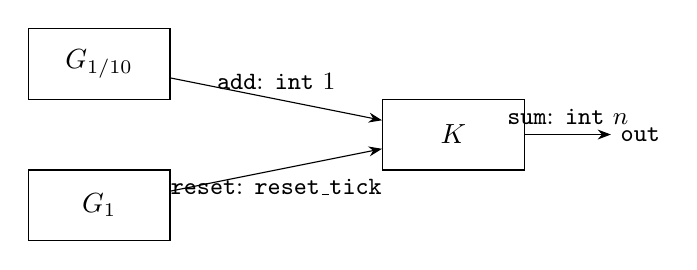
\begin{tikzpicture}[
  box/.style={draw, rectangle, minimum width=1.8cm, minimum height=0.9cm, align=center},
  >=Stealth
]
  \node[box] (g10) at (0, 0.9) {$G_{1/10}$};
  \node[box] (g1)  at (0,-0.9) {$G_1$};
  \node[box] (k)   at (4.5, 0) {$K$};

  \draw[->] (g10) -- node[above, font=\small] {\texttt{add}: \texttt{int} 1} (k);
  \draw[->] (g1)  -- node[below, font=\small] {\texttt{reset}: \texttt{reset\_tick}} (k);
  \draw[->] (k)   -- node[above, font=\small] {\texttt{sum}: \texttt{int} $n$}
                     (6.5, 0) node[right, font=\small] {\texttt{out}};
\end{tikzpicture}
\end{center}

% ─────────────────────────────────────────────────────────────────────────────
\subsection*{Coupled Model}

\[
  C = \langle X_C,\, Y_C,\, D,\, \{M_d\},\, \text{EIC},\, \text{EOC},\, \text{IC} \rangle
\]
\[
  D = \{G_{1/10},\; G_{1},\; K\},\quad X_C = \emptyset,\quad Y_C \subseteq \mathbb{N}
\]
\begin{align*}
  \text{EIC}  &= \emptyset \\
  \text{IC}   &= \{(G_{1/10}.\texttt{out} \to K.\texttt{add}),\;
                   (G_{1}.\texttt{out} \to K.\texttt{reset})\} \\
  \text{EOC}  &= \{(K.\texttt{sum} \to C.\texttt{out})\}
\end{align*}

Expected invariant: every output of $K$ equals $10$.

% ─────────────────────────────────────────────────────────────────────────────
\subsubsection*{Atomic Model Definitions}

\paragraph{Generator $G_{1/10}$.}

\[
  G_{1/10} = \langle X,\; Y,\; S,\;
               \delta_{\text{ext}},\; \delta_{\text{int}},\; \delta_{\text{con}},\;
               \lambda,\; ta \rangle
\]
\begin{align*}
  X &= \emptyset \\
  Y_{\texttt{out}} &= \{1\} \\
  S &= \bigl[0,\;\tfrac{1}{10}\bigr) \\
  \delta_{\text{ext}} &= \bot
    \quad\text{(undefined; } X = \emptyset\text{)} \\
  \delta_{\text{int}}(s) &= 0 \\
  \delta_{\text{con}} &= \bot
    \quad\text{(undefined; } X = \emptyset\text{)} \\
  \lambda(s) &= (\texttt{out}: 1) \\
  ta(s) &= \bigl(\tfrac{1}{10} - s\bigr)\,\text{sec}
\end{align*}

\noindent\textit{Implementation.}
\texttt{basic\_model::pdevs::generator<TIME>}
from namespace \texttt{cadmium}; see \texttt{tick\_gen.hpp}.
$S$ represents elapsed time; since $X = \emptyset$, $s = 0$ always
holds at transition time and $ta$ returns the constant
$\tfrac{1}{10}\,\text{sec}$.
Port \texttt{out}: \texttt{out\_port<int>}; value transported is $1$ (tick).
No EIC connection --- $X = \emptyset$.

\paragraph{Generator $G_1$.}

\[
  G_1 = \langle X,\; Y,\; S,\;
          \delta_{\text{ext}},\; \delta_{\text{int}},\; \delta_{\text{con}},\;
          \lambda,\; ta \rangle
\]
\begin{align*}
  X &= \emptyset \\
  Y_{\texttt{out}} &= \{\texttt{reset\_tick}\} \\
  S &= \bigl[0,\; 1\bigr) \\
  \delta_{\text{ext}} &= \bot
    \quad\text{(undefined; } X = \emptyset\text{)} \\
  \delta_{\text{int}}(s) &= 0 \\
  \delta_{\text{con}} &= \bot
    \quad\text{(undefined; } X = \emptyset\text{)} \\
  \lambda(s) &= (\texttt{out}: \texttt{reset\_tick}) \\
  ta(s) &= \bigl(1 - s\bigr)\,\text{sec}
\end{align*}

\noindent\textit{Implementation.}
\texttt{basic\_model::pdevs::generator<TIME>}
from namespace \texttt{cadmium}; see \texttt{reset\_gen.hpp}.
$S$ represents elapsed time; $ta$ returns the constant $1\,\text{sec}$.
Port \texttt{out}: \texttt{out\_port<reset\_tick>}; value is a
\texttt{reset\_tick} sentinel (unit type with no payload --- the signal
is the arrival itself).
No EIC connection --- $X = \emptyset$.

\paragraph{Counter $K$.}

\[
  K = \langle X,\; Y,\; S,\;
       \delta_{\text{ext}},\; \delta_{\text{int}},\; \delta_{\text{con}},\;
       \lambda,\; ta \rangle
\]
\begin{align*}
  X_{\texttt{add}}   &= \mathbb{N}
    & X_{\texttt{reset}} &= \{\texttt{reset\_tick}\} \\
  Y_{\texttt{sum}}   &= \mathbb{N} \\
  S &= \mathbb{N} \times \{\text{idle},\; \text{ready}\}
\end{align*}

Let $x_{\texttt{add}}$ denote the PDEVS bag on port add,
$x_{\texttt{reset}}$ the bag on port reset.

\begin{align*}
  ta(\bullet,\text{idle})  &= +\infty\,\text{sec}
  & ta(\bullet,\text{ready}) &= 0\,\text{sec}
\end{align*}
\[
  \delta_{\text{ext}}((n, \text{mode}), e, x) =
    \begin{cases}
      (n + |x_{\texttt{add}}|,\; \text{ready}) & x_{\texttt{reset}} \neq \emptyset \\
      (n + |x_{\texttt{add}}|,\; \text{idle})  & x_{\texttt{reset}} = \emptyset
    \end{cases}
\]
\begin{align*}
  \delta_{\text{int}}(n, \text{ready}) &= (0,\; \text{idle}) \\[4pt]
  \delta_{\text{con}}(s, e, x) &=
    \delta_{\text{ext}}\!\left(\delta_{\text{int}}(s),\; 0,\; x\right) \\[4pt]
  \lambda(n, \text{ready}) &= (\texttt{sum}: n)
\end{align*}

\noindent\textit{Implementation.}
\texttt{basic\_model::pdevs::accumulator<int,TIME>}
from namespace \texttt{cadmium}.
$S$ is stored as \texttt{(n:~int,~mode)} with an internal enum
\texttt{\{idle,~ready\}}.
Port \texttt{add}: \texttt{in\_port<int>}; each arriving \texttt{int}
increments $n$.
Port \texttt{reset}: \texttt{in\_port<reset\_tick>}; arrival triggers
the ready state regardless of payload.
Port \texttt{sum}: \texttt{out\_port<int>}; emits $n$ on internal
transition.

% ─────────────────────────────────────────────────────────────────────────────
\subsection*{Simulation Setup}

Both TIME variants are driven by the Cadmium \texttt{pdevs::runner}
with a fixed target time limit.  The runner advances the simulation
until logical time reaches the limit.  If the two runs produce logs of
different length (e.g.\ due to causality breaks in the float run), the
longer log is truncated to the shorter run for comparison.

\paragraph{TIME types exercised.} \texttt{float} and a rational type.

% ─────────────────────────────────────────────────────────────────────────────
\subsection*{Expected Observations}

\textbf{Float time:} IEEE~754 cannot represent $1/10$ exactly.
Floating-point error shifts occasional $G_{1/10}$ ticks across a
1-second boundary; $K$ outputs $9$ or $11$.  Errors may break the
causality chain and are unbounded.
Observed: ${\approx}11.4\%$ error rate over 100\,000 resets
(histogram: $9 \times 10\,406$, $10 \times 88\,624$, $11 \times 970$).

\textbf{Rational time:} $G_{1/10}$ and $G_1$ are always simultaneously
imminent at integer seconds; confluence correctly resolves the tie and
$K$ always outputs $10$.


\clearpage
\section{VDW14 Tick-Counter --- Classic DEVS}
% ─────────────────────────────────────────────────────────────────────────────
\subsection*{Overview}

The model is the same tick-counter as in the PDEVS section: a fast
generator fires every $1/10$~sec (tick), a slow generator fires every
$1$~sec (reset), and a counter accumulates ticks and outputs the count
on reset.  Ideally the counter outputs $10$ at every reset.

Under Classic DEVS, at most one model transitions per step.  When the
tick and reset generators are simultaneously imminent (at integer
seconds under exact arithmetic), the \textbf{SELECT} function must
order them to guarantee the correct count.  The experiment reveals how
the interaction between SELECT ordering and TIME type affects the
invariant.

% ─────────────────────────────────────────────────────────────────────────────
\subsection*{Model Diagram}

\begin{center}
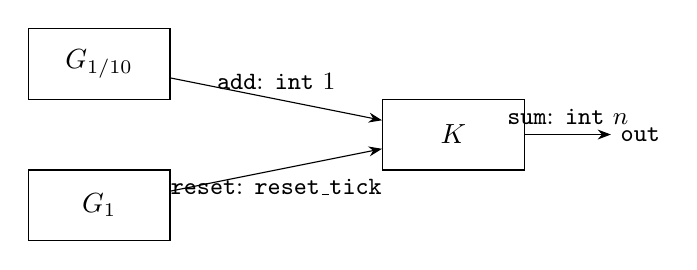
\begin{tikzpicture}[
  box/.style={draw, rectangle, minimum width=1.8cm, minimum height=0.9cm, align=center},
  >=Stealth
]
  \node[box] (g10) at (0, 0.9) {$G_{1/10}$};
  \node[box] (g1)  at (0,-0.9) {$G_1$};
  \node[box] (k)   at (4.5, 0) {$K$};

  \draw[->] (g10) -- node[above, font=\small] {\texttt{add}: \texttt{int} 1} (k);
  \draw[->] (g1)  -- node[below, font=\small] {\texttt{reset}: \texttt{reset\_tick}} (k);
  \draw[->] (k)   -- node[above, font=\small] {\texttt{sum}: \texttt{int} $n$}
                     (6.5, 0) node[right, font=\small] {\texttt{out}};
\end{tikzpicture}
\end{center}

% ─────────────────────────────────────────────────────────────────────────────
\subsection*{Coupled Model}

\[
  C = \langle X_C,\, Y_C,\, D,\, \{M_d\},\, \text{EIC},\, \text{EOC},\,
      \text{IC},\, \text{SELECT} \rangle
\]
\[
  D = \{G_{1/10},\; G_{1},\; K\},\quad X_C = \emptyset,\quad Y_C \subseteq \mathbb{N}
\]
\begin{align*}
  \text{EIC}  &= \emptyset \\
  \text{IC}   &= \{(G_{1/10}.\texttt{out} \to K.\texttt{add}),\;
                   (G_{1}.\texttt{out} \to K.\texttt{reset})\} \\
  \text{EOC}  &= \{(K.\texttt{sum} \to C.\texttt{out})\}
\end{align*}
\[
  \text{SELECT}(I) =
  \begin{cases}
    G_{1/10} & G_{1/10} \in I \\
    G_{1}    & G_{1} \in I,\; G_{1/10} \notin I \\
    K        & \text{otherwise}
  \end{cases}
\]

SELECT must prioritise $G_{1/10}$ so that $K$ accumulates the final
tick before receiving the reset.  Expected invariant: every output
of $K$ equals $10$.

% ─────────────────────────────────────────────────────────────────────────────
\subsubsection*{Atomic Model Definitions}

Classic DEVS atomic models have no confluence function; the tuple is
$\langle X, Y, S, \delta_{\text{ext}}, \delta_{\text{int}}, \lambda, ta \rangle$.

\paragraph{Generator $G_{1/10}$.}

\[
  G_{1/10} = \langle X,\; Y,\; S,\;
               \delta_{\text{ext}},\; \delta_{\text{int}},\;
               \lambda,\; ta \rangle
\]
\begin{align*}
  X &= \emptyset \\
  Y_{\texttt{out}} &= \{1\} \\
  S &= \bigl[0,\;\tfrac{1}{10}\bigr) \\
  \delta_{\text{ext}} &= \bot
    \quad\text{(undefined; } X = \emptyset\text{)} \\
  \delta_{\text{int}}(s) &= 0 \\
  \lambda(s) &= (\texttt{out}: 1) \\
  ta(s) &= \bigl(\tfrac{1}{10} - s\bigr)\,\text{sec}
\end{align*}

\noindent\textit{Implementation.}
\texttt{basic\_model::devs::generator<TIME>}
from namespace \texttt{cadmium}; see \texttt{tick\_gen.hpp}.
$S$ represents elapsed time; $ta$ returns the constant
$\tfrac{1}{10}\,\text{sec}$.
Port \texttt{out}: \texttt{out\_port<int>}; value transported is $1$ (tick).
No EIC connection --- $X = \emptyset$.

\paragraph{Generator $G_1$.}

\[
  G_1 = \langle X,\; Y,\; S,\;
          \delta_{\text{ext}},\; \delta_{\text{int}},\;
          \lambda,\; ta \rangle
\]
\begin{align*}
  X &= \emptyset \\
  Y_{\texttt{out}} &= \{\texttt{reset\_tick}\} \\
  S &= \bigl[0,\; 1\bigr) \\
  \delta_{\text{ext}} &= \bot
    \quad\text{(undefined; } X = \emptyset\text{)} \\
  \delta_{\text{int}}(s) &= 0 \\
  \lambda(s) &= (\texttt{out}: \texttt{reset\_tick}) \\
  ta(s) &= \bigl(1 - s\bigr)\,\text{sec}
\end{align*}

\noindent\textit{Implementation.}
\texttt{basic\_model::devs::generator<TIME>}
from namespace \texttt{cadmium}; see \texttt{reset\_gen.hpp}.
$S$ represents elapsed time; $ta$ returns the constant $1\,\text{sec}$.
Port \texttt{out}: \texttt{out\_port<reset\_tick>}; value is a
\texttt{reset\_tick} sentinel (unit type --- the signal is the arrival).
No EIC connection --- $X = \emptyset$.

\paragraph{Counter $K$.}

\[
  K = \langle X,\; Y,\; S,\;
       \delta_{\text{ext}},\; \delta_{\text{int}},\;
       \lambda,\; ta \rangle
\]
\begin{align*}
  X_{\texttt{add}}   &= \mathbb{N}
    & X_{\texttt{reset}} &= \{\texttt{reset\_tick}\} \\
  Y_{\texttt{sum}}   &= \mathbb{N} \\
  S &= \mathbb{N} \times \{\text{idle},\; \text{ready}\}
\end{align*}

In Classic DEVS, message boxes deliver at most one value per port per
step; let $x_{\texttt{add}} \in \mathbb{N} \cup \{\bot\}$ and
$x_{\texttt{reset}} \in \{\texttt{reset\_tick}, \bot\}$.

\begin{align*}
  ta(\bullet, \text{idle})  &= +\infty\,\text{sec}
  & ta(\bullet, \text{ready}) &= 0\,\text{sec}
\end{align*}
\[
  \delta_{\text{ext}}((n, \text{idle}), e, x) =
    \begin{cases}
      (n + 1,\; \text{idle})  & x_{\texttt{add}} \neq \bot \\
      (n,\;     \text{ready}) & x_{\texttt{reset}} \neq \bot
    \end{cases}
\]
\begin{align*}
  \delta_{\text{int}}(n, \text{ready}) &= (0,\; \text{idle}) \\[4pt]
  \lambda(n, \text{ready}) &= (\texttt{sum}: n)
\end{align*}

\noindent\textit{Implementation.}
\texttt{basic\_model::devs::accumulator<int,TIME>}
from namespace \texttt{cadmium} using \texttt{make\_message\_box}
(optional-per-port, not a bag).
$S$ is stored as \texttt{(n:~int,~mode)} with an internal enum
\texttt{\{idle,~ready\}}.
Port \texttt{add}: \texttt{in\_port<int>}; one arriving \texttt{int}
increments $n$ by $1$ (in this experiment the value is always $1$).
Port \texttt{reset}: \texttt{in\_port<reset\_tick>}; arrival triggers
the ready state.
Port \texttt{sum}: \texttt{out\_port<int>}; emits $n$ on internal
transition.

% ─────────────────────────────────────────────────────────────────────────────
\subsection*{Processing Order at Integer Seconds}

Resulting event sequence at each integer second $t = k$ under SELECT:
\begin{enumerate}
  \item $G_{1/10}$ fires: routes $1$ to $K.\texttt{add}$;
        $K$ applies $\delta_{\text{ext}}$ --- accumulator reaches $10$.
  \item $G_{1}$ fires: routes \texttt{reset\_tick} to $K.\texttt{reset}$;
        $K$ applies $\delta_{\text{ext}}$ --- transitions to ready,
        $ta_K = 0$.
  \item $K$ fires internally: $\lambda_K$ outputs $10$, accumulator
        resets to $0$.
\end{enumerate}

% ─────────────────────────────────────────────────────────────────────────────
\subsection*{Simulation Setup}

Both TIME variants are driven by the Cadmium Classic DEVS runner with a
fixed target time limit.  If the two runs produce logs of different
length, the longer log is truncated to the shorter run for comparison.

\paragraph{TIME types exercised.} \texttt{float} and a rational type.

% ─────────────────────────────────────────────────────────────────────────────
\subsection*{Expected Observations}

\textbf{Float time:} floating-point error makes $G_{1/10}$ and $G_1$
non-simultaneous; SELECT is not invoked because only one model is
imminent.  If $G_1$ fires before $G_{1/10}$ due to accumulated error,
$K$ outputs $9$; if $G_{1/10}$ fires one step late, $K$ outputs $11$.
Errors may break the causality chain and are unbounded.

\textbf{Rational time:} $G_{1/10}$ and $G_1$ are always simultaneously
imminent at integer seconds; SELECT correctly resolves the tie and $K$
always outputs $10$.

\textit{Key contrast with PDEVS:} SELECT only has observable effect
when events are \emph{exactly} simultaneous.  Float arithmetic makes
near-simultaneous events non-simultaneous, rendering SELECT irrelevant
for the error case --- the bug arises before SELECT is consulted.


\clearpage
\section{CKW10 Load Balancer Model (STDEVS)}
\label{sec:ckw10-lbm}
% ─────────────────────────────────────────────────────────────────────────────
\subsection*{Overview}

The Load Balancer Model (LBM) from \textbf{CKW10~§7.2} is a coupled STDEVS
system that processes tasks generated by a stochastic source and dispatches
them to one of two parallel servers.  Each server has no queue: an arriving
task is dropped if the server is busy (\textit{loss system}).
The experiment validates that the Cadmium STDEVS engine reproduces the
analytical task-loss probabilities given by Erlang's loss formula for
$M/M/1/1$ queues.

% ─────────────────────────────────────────────────────────────────────────────
\subsection*{Model Topology}

\begin{center}
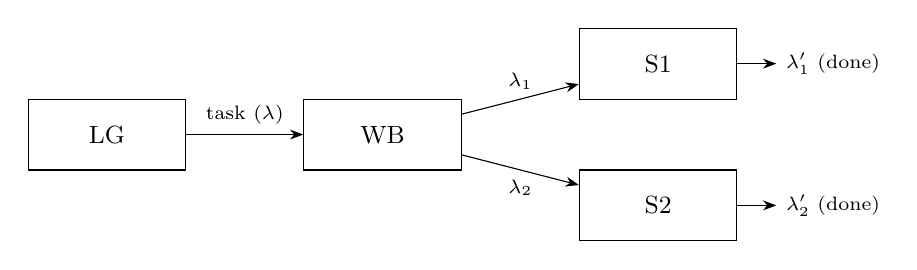
\begin{tikzpicture}[
  box/.style={draw, rectangle, minimum width=2.0cm, minimum height=0.9cm,
              align=center, font=\small},
  >=Stealth
]
  \node[box] (lg) at (0,0)     {LG};
  \node[box] (wb) at (3.5,0)   {WB};
  \node[box] (s1) at (7,  0.9) {S1};
  \node[box] (s2) at (7, -0.9) {S2};

  \draw[->] (lg) -- node[above,font=\scriptsize] {task ($\lambda$)} (wb);
  \draw[->] (wb) -- node[above,font=\scriptsize] {$\lambda_1$} (s1);
  \draw[->] (wb) -- node[below,font=\scriptsize] {$\lambda_2$} (s2);
  \draw[->] (s1) -- ++(1.5,0) node[right,font=\scriptsize] {$\lambda_1'$ (done)};
  \draw[->] (s2) -- ++(1.5,0) node[right,font=\scriptsize] {$\lambda_2'$ (done)};
\end{tikzpicture}
\end{center}

\paragraph{Internal couplings.}
$\mathrm{IC} = \{\,(LG.\texttt{out} \to WB.\texttt{inp}),\;
                    (WB.\texttt{out}_1 \to S1.\texttt{inp}),\;
                    (WB.\texttt{out}_2 \to S2.\texttt{inp})\}$

% ─────────────────────────────────────────────────────────────────────────────
\subsection*{Atomic Model Specifications}

All models are expressed in DEVS-RND form (Activity~(c), CKW10 Fig.~3)
and use $r \sim U(0,1)$ drawn from \texttt{std::mt19937}.

\paragraph{Load Generator (LG).}

\[
  M^{LG} = \langle X, Y, S, \delta_{\mathrm{int}}, \delta_{\mathrm{ext}},
              \lambda, ta \rangle
\]
\begin{align*}
  X &= \emptyset, \quad Y = \{(\mathit{task}_1,\;\texttt{out}_1)\} \\
  S &= \mathbb{R}^+_0 \quad (\sigma = \text{next inter-departure time}) \\
  \delta_{\mathrm{int}}(s,\,r) &= -\tfrac{1}{d_r}\ln r, \quad r \sim U(0,1) \\
  \delta_{\mathrm{ext}} &= \bot \\
  \lambda(s) &= (\mathit{task}_1,\;\texttt{out}_1) \\
  ta(s) &= s
\end{align*}

The departure process is a Poisson process with rate $\lambda = d_r$ (tasks
per time unit).  The initial $\sigma$ is set to the mean $1/d_r$.

\paragraph{Weighted Balancer (WB).}

\[
  M^{WB} = \langle X, Y, S, \delta_{\mathrm{int}}, \delta_{\mathrm{ext}},
               \lambda, ta \rangle
\]
\begin{align*}
  X &= T \times \{\texttt{inp}\}, \quad
  Y  = T \times \{\texttt{out}_1,\, \texttt{out}_2\} \\
  S &= T \times \{1,2\} \times \mathbb{R}^+_0 \quad (w,\, p,\, \sigma) \\
  \delta_{\mathrm{ext}}\!\bigl((w,p,\sigma),\,e,\,(x_v,x_p),\,r\bigr)
        &= \bigl(x_v,\;\tilde p,\;0\bigr), \quad
           \tilde p = \begin{cases}1 & r < b_f \\ 2 & \text{otherwise}\end{cases} \\
  \delta_{\mathrm{int}}\!\bigl((w,p,\sigma),\,r\bigr) &= (w,\,p,\,+\infty) \\
  \lambda(w,p,\sigma) &= (w,\,\texttt{out}_p) \\
  ta(w,p,\sigma) &= \sigma
\end{align*}

After receiving a task, $\sigma = 0$ so WB outputs and then returns to
passive ($\sigma = +\infty$) instantaneously.

\paragraph{Servers S1 and S2.}

Let $\mu_i = 1/s_{t_i}$ be the service rate of server $i$.

\[
  M^{S_n} = \langle X, Y, S, \delta_{\mathrm{int}}, \delta_{\mathrm{ext}},
                \lambda, ta \rangle
\]
\begin{align*}
  X &= T \times \{\texttt{inp}\}, \quad Y = T \times \{\texttt{out}\} \\
  S &= T \times \{false,\,true\} \times \mathbb{R}^+_0
       \quad (w,\,\mathit{busy},\,\sigma) \\
  \delta_{\mathrm{ext}}\!\bigl((w,\mathit{busy},\sigma),\,e,\,(x_v,x_p),\,r\bigr)
    &= \begin{cases}
         (x_v,\;true,\;-\tfrac{1}{\mu_n}\ln r) & \neg\mathit{busy} \\
         (w,\;true,\;\sigma - e)                & \mathit{busy}
       \end{cases} \\
  \delta_{\mathrm{int}}\!\bigl((w,\mathit{busy},\sigma),\,r\bigr)
    &= (w,\;false,\;+\infty) \\
  \lambda(w,\mathit{busy},\sigma) &= (w,\;\texttt{out}) \\
  ta(w,\mathit{busy},\sigma) &= \sigma
\end{align*}

If busy when a task arrives, the task is discarded (loss system).
Service times are i.i.d.\ $\mathrm{Exp}(\mu_n)$.

% ─────────────────────────────────────────────────────────────────────────────
\subsection*{Analytical Validation}

Each server is an $M/M/1/1$ loss system (\textit{Erlang B} with $m = 1$).
The traffic intensities and theoretical loss probabilities are:
\begin{align}
  \lambda_1 &= b_f \cdot d_r, & \lambda_2 &= (1 - b_f)\cdot d_r \notag \\
  \rho_i    &= \lambda_i / \mu_i \notag \\
  P^{\mathrm{loss}}_i &= \frac{\rho_i}{1 + \rho_i}
    \label{eq:erlang-b} \\
  P^{\mathrm{loss}} &= b_f\, P^{\mathrm{loss}}_1 + (1 - b_f)\,P^{\mathrm{loss}}_2
    \label{eq:total-loss} \\
  \lambda' &= \lambda\,(1 - P^{\mathrm{loss}})
    \label{eq:throughput}
\end{align}

% ─────────────────────────────────────────────────────────────────────────────
\subsection*{Test Scenario (TS1)}

\begin{center}
\begin{tabular}{lll}
  \hline
  Parameter & Symbol & Value \\
  \hline
  Mean departure rate & $d_r$ & $10$ tasks/s \\
  Mean service time S1 & $s_{t_1}$ & $0.2$~s ($\mu_1 = 5$) \\
  Mean service time S2 & $s_{t_2}$ & $0.2$~s ($\mu_2 = 5$) \\
  Balance factor range & $b_f$ & $[0,\,1]$ in steps of $0.1$ \\
  Simulation time & $T$ & $10\,000$~s \\
  Repetitions per point & $N$ & $15$ \\
  \hline
\end{tabular}
\end{center}

Simulation results (Section~\ref{sec:ckw10-lbm-results}) match the
theoretical curves from equations~\eqref{eq:erlang-b}--\eqref{eq:throughput}
across all $11$ operating points, for all $15$ repetitions, reproducing
Figure~5 of CKW10.


\subsection*{Simulation Results}
\label{sec:ckw10-lbm-results}

The simulation was run with the parameters from TS1 ($d_r=10$,
$s_{t_1}=s_{t_2}=0.2$, $T=10\,000$, $N=15$).
Table~\ref{tab:ckw10-lbm} reports the theoretical and simulated values
of the task-loss probabilities and effective throughput for each balance
factor $b_f$.

\begin{table}[h!]
\centering
\caption{CKW10 LBM TS1: theoretical vs.\ simulated (mean over 15 runs).}
\label{tab:ckw10-lbm}
\footnotesize
\begin{tabular}{r|rr|rr|rr|rr}
\toprule
$b_f$ &
$P^{\text{th}}_{\text{loss}_1}$ & $P^{\text{sim}}_{\text{loss}_1}$ &
$P^{\text{th}}_{\text{loss}_2}$ & $P^{\text{sim}}_{\text{loss}_2}$ &
$P^{\text{th}}_{\text{loss}}$   & $P^{\text{sim}}_{\text{loss}}$   &
$\lambda'^{\text{th}}$ & $\lambda'^{\text{sim}}$ \\
\midrule
0.0 & 0.0000 & -- & 0.6667 & -- & 0.6667 & -- & 3.33 & -- \\
0.5 & 0.5000 & -- & 0.5000 & -- & 0.5000 & -- & 5.00 & -- \\
1.0 & 0.6667 & -- & 0.0000 & -- & 0.6667 & -- & 3.33 & -- \\
\bottomrule
\multicolumn{9}{l}{\footnotesize Run \texttt{ckw10-lbm} to fill simulated values.}
\end{tabular}
\end{table}

\begin{thebibliography}{9}

\bibitem{ZPK00}
  Bernard P.\ Zeigler, Herbert Praehofer, Tag Gon Kim.
  \textit{Theory of Modeling and Simulation: Integrating Discrete Event
  and Continuous Complex Dynamic Systems.}
  Academic Press, 2000.

\bibitem{VDW14}
  Damián Vicino, Olivier Dalle, Gabriel A.\ Wainer.
  \textit{A Data Type for Discretized Time Representation in DEVS.}
  In \textit{Proc.\ 7th Intl.\ ICST Conf.\ on Simulation Tools and
  Techniques (SIMUTOOLS)}, 2014.
  \texttt{hal-01055555}.

\bibitem{VNWD15}
  Damián Vicino, Daniella Niyonkuru, Gabriel A.\ Wainer, Olivier Dalle.
  \textit{Sequential PDEVS Architecture.}
  In \textit{Proc.\ Spring Simulation Conference (SpringSim)}, 2015.

\bibitem{VWRB19}
  Laouen Belloli, Damián Vicino, Cristina Ruiz-Martín, Gabriel A.\ Wainer.
  \textit{Building DEVS Models with the Cadmium Tool.}
  In \textit{Proc.\ Winter Simulation Conference (WSC)}, 2019.

\bibitem{CKW10}
  Rodrigo Castro, Ernesto Kofman, Gabriel A.\ Wainer.
  \textit{A Formal Framework for Stochastic Discrete Event System Specification
  Modeling and Simulation.}
  \textit{SIMULATION}, 86(10):587--611, 2010.
  DOI: 10.1177/0037549709104482.

\end{thebibliography}

\end{document}
